\documentclass[20pt]{report}
\usepackage{makeidx}
\usepackage{graphicx}
\usepackage{amsmath}
\graphicspath{ {./images/} }

\begin{document}

\begin{titlepage}
\author{\Large Hanan Basheer} 
\title{Quantum Information and Computing\\
\textit{\Large Summer of Science '22}} 
\date{}
\maketitle
\end{titlepage}

\tableofcontents{}

\part{Introduction}
\index{Introduction}
\textbf{Quantum computation and Quantum Information} is the study of the information processing tasks that can be accomplished using a quantum mechanical system. 
\par A series of crises had arisen in physics in the 20th Century. The problem was that the theories of physics at that time (now dubbed classical physics) were predicting absurdities such as the existence of an ‘ultraviolet catastrophe’ involving infinite energies, or electrons spiralling inexorably into the atomic nucleus. At first, such problems were resolved by adding ad hoc hypotheses to classical physics, but as a better understanding of atoms and radiation was gained these attempted explanations became more and more convoluted. The crisis came to a head in the early 1920s after a quarter-century of turmoil and resulted in the creation of the modern theory of \textit{quantum mechanics}.
\par
\textbf{Quantum mechanics} is a mathematical framework or set of rules for the construction of physical theories. The rules of quantum mechanics are simple but even experts find them counterintuitive, and the earliest antecedents of quantum computation and quantum information may be found in the long-standing desire of physicists to better understand quantum mechanics. 
\par One paradigm is provided by the theory of quantum computation, which is based on the idea of using quantum mechanics to perform computations, instead of classical physics. It turns out that while an ordinary computer can be used to simulate a quantum computer, it appears to be impossible to perform the simulation in an efficient fashion. Thus quantum computers offer an essential speed advantage over classical computers. This speed advantage is so significant that many researchers believe that no conceivable amount of progress in classical computation would be able to overcome the gap between the power of a classical computer and the power of a quantum computer.
\par
The remarkable first step taken by Deutsch, in proposing an example showing quantum computers might have computational powers exceeding those of classical computer, was improved in the subsequent decade by many people, culminating in Peter Shor’s 1994 demonstration that two enormously important problems – the problem of finding the prime factors of an integer, and the so-called ‘discrete logarithm’ problem – could be solved efficiently on a quantum computer. This attracted widespread interest because these two problems were and still are widely believed to have no efficient solution on a classical computer. Shor’s results are a powerful indication that quantum computers are more powerful than Turing machines, even probabilistic Turing machines.
\par
At the same time computer science was exploding in the 1940s, another revolution was taking place in our understanding of communication. In 1948 Claude Shannon published a remarkable pair of papers laying the foundations for the modern theory of information and communication. This was the beginning of \textbf{Information Theory}. Perhaps the key step taken by Shannon was to mathematically define the concept of \textit{information}. The first, Shannon’s noiseless channel coding theorem, quantifies
the physical resources required to store the output from an information source. Shannon’s second fundamental theorem, the noisy channel coding theorem, quantifies how much information it is possible to reliably transmit through a noisy communications channel.
\par
Quantum information theory has followed with similar developments. In 1995, Ben Schumacher provided an analogue to Shannon’s noiseless coding theorem, and in the process defined the ‘quantum bit’ or ‘qubit’ as a tangible physical resource. However, no analogue to Shannon’s noisy channel coding theorem is yet known for quantum information. Nevertheless, in analogy to their classical counterparts, a theory of quantum error-correction has been developed which, as already mentioned, allows quantum computers to compute effectively in the presence of noise, and also allows communication over noisy quantum channels to take place reliably. The theory of quantum error-correcting codes was developed to protect quantum states
against noise.
\par
One of the earliest discoveries in quantum computation and quantum information was that quantum mechanics can be used to do key distribution in such a way that security of the parties trying to communicate can not be compromised. This procedure is known as \textbf{Quantum Cryptography} or quantum key distribution. The basic idea is to exploit the quantum mechanical principle that observation in general disturbs the system being observed. Thus, if there is an eavesdropper listening in as two parties attempt to transmit their key, the presence of the eavesdropper will be visible as a disturbance of the communications channel which the parties are using to establish the key. These parrties can then throw out the key bits established while the eavesdropper was listening in, and start over.
\par
Perhaps the most striking of these is the study of \textbf{Quantum Entanglement}. Entanglement is a uniquely quantum mechanical resource that plays a key role in many of the most interesting applications of quantum computation and quantum information. In recent years there has been a tremendous effort trying to better understand the properties of entanglement considered as a fundamental resource of Nature, of comparable importance to energy, information, entropy, or any other fundamental resource.

\part{Quantum Bits and Computation}
\index{Quantum Bits and Computation}
The \textit{bit} is the fundamental concept of classical computation and classical information.
Quantum computation and quantum information are built upon an analogous concept,
the \textit{quantum bit}, or \textit{qubit} for short. In this section we introduce the properties of single
and multiple qubits, comparing and contrasting their properties to those of classical bits.
\par
Just as a classical bit has a state – either 0 or 1 – a qubit also
has a state. Two possible states for a qubit are the states $|0\rangle$ and $|1\rangle$, which as you might
guess correspond to the states 0 and 1 for a classical bit. Notation like ‘$| \rangle$’ is called the
\textit{Dirac notation}.  The difference between bits and qubits is that a qubit can be in a
state other than $|0\rangle $ or $|1\rangle$. It is also possible to form linear combinations of states, often
called \textit{superpositions}: 
\begin{equation}
|\psi = \alpha|0\rangle + \beta|1\rangle
\end{equation}
\par
We can examine a bit to determine whether it is in the state 0 or 1. For example,
computers do this all the time when they retrieve the contents of their memory. Rather
remarkably, we cannot examine a qubit to determine its quantum state, that is, the
values of $\alpha$ and $\beta$. Instead, quantum mechanics tells us that we can only acquire much more restricted information about the quantum state.
\par
The ability of a qubit to be in a superposition state runs counter to our ‘common sense’
understanding of the physical world around us. A classical bit is like a coin: either heads
or tails up. For imperfect coins, there may be intermediate states like having it balanced
on an edge, but those can be disregarded in the ideal case. By contrast, a qubit can exist
in a continuum of states between $|0\rangle$ and $|1\rangle$ – until it is observed. Let us emphasize
again that when a qubit is measured, it only ever gives ‘0’ or ‘1’ as the measurement
result – probabilistically. For example, a qubit can be in the state
\begin{equation}
\frac{1}{\sqrt{2}}|0\rangle + \frac{1}{\sqrt{2}}|1\rangle
\end{equation}
One picture useful in thinking about qubits is the following geometric representation. Because $|\alpha|^2 + |\beta|^2 = 1$, we may rewrite Equation (1) as
\begin{equation}
|\psi\rangle = \cos{\frac{\theta}{2}}|0\rangle + e^{i\phi} \sin{\frac{\theta}{2}}|1\rangle
\end{equation}
The numbers $\theta$ and $\phi$ define a point on the unit three-dimensional sphere. This sphere is often called the \textit{Bloch sphere}. It provides a useful means of visualizing the state of a single qubit.\\
\begin{center}
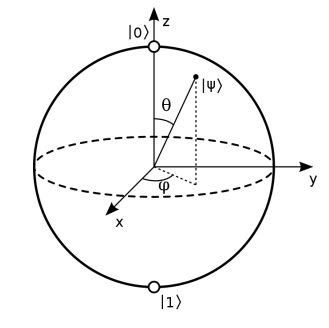
\includegraphics[width=5cm]{Sphere} \\
\textit{Bloch Sphere representation of a Qubit} \\
\end{center}
We observe that Postulate 2 of Quantum Mechanics, describes how a closed system evolves through a unitary operator. An equivalent view of this postulate, the Schr$\ddot{o}$dinger Equation, describes the system evolution in
continuous-time,
\begin{equation}
i\hbar \frac{d |\psi\rangle}{dt} = H |\psi\rangle
\end{equation}
Here, H is a Hermitian operator known as the Hamiltonian of the system. The solution to the equation can be written as,
\begin{equation}
|\psi(t2)\rangle = e^{-i \frac{H(t_{2}-t_{1})}{\hbar}}|\psi(t_{1})\rangle = U(t_{1}, t_{2})|\psi(t_{1})\rangle
\end{equation}
where we define,
\begin{equation}
U(t_{2}, t_{1}) = e^{-i \frac{H(t_{2}-t_{1})}{\hbar}}
\end{equation}
In fact, this is just a special case of a useful result: any unitary operator U can be written as $U = exp(iK)$, where K is a Hermitian matrix. This bridges the gap between the discrete-time representation (Postulate 2) and Schr$\ddot{o}$dinger’s equation. \\

It is important to emphasize that Postulate 2 describes the evolution of a closed quantum system. However, when we make a measurement on the system, this counts as an external interaction. Post-measurement, the state of the system is described by Postulate 3. Given our collection of measurement operators $M_{m}$ operating on a system in a state $|\psi\rangle$ prior to the measurement, the probability that result m is measured is,
\begin{equation}
p(m) = \langle\psi|M_{m}^{+}M_{m}|\psi\rangle
\end{equation}
and the state of the system post-measurement is,
\begin{equation}
|\psi ' \rangle = \frac{M_{m} |\psi\rangle}{\sqrt{\langle\psi|M_{m}^{+}M_{m}|\psi\rangle}}
\end{equation}
Note that for normalized probabilities, we require that {Mm} satisfy the completeness relation. An example depicting the use of measurements is the measurement of a qubit in the computational basis. We have two measurement operators $M_{0}$ = $|0\rangle \langle0|$ and $M_{1}$ = $|1\rangle \langle0|$. We can see that for a state $|\psi\rangle = a |0\rangle + b |1\rangle$, the state post measurement is,
\begin{center}
$\frac{a}{|a|}|0\rangle$ with probability p(0) = $|a|^2$ \\
$\frac{b}{|b|}|0\rangle$ with probability p(1) = $|b|^2 $\\
\end{center}
There is also a special class of measurements, known as projective measurements, which are described
by an observable M, which is a Hermitian operator having a spectral decomposition,
$M = \sum_{m}mP_{m}$, where Pm is the projector onto the eigenspace of M with eigenvalue m. The probability of obtaining
the result m upon measuring the state $|\psi\rangle$ is given by,
\begin{equation}
p(m) = \langle\psi|P_{m}|\psi\rangle
\end{equation}
and the state post-measurement is
\begin{equation}
|\psi ' \rangle = \frac{P_{m}|\psi\rangle}{\sqrt{p(m)}}
\end{equation}
Using equation 7, we can the obtain the average value $\langle M \rangle$ of the observable as,
\begin{equation}
\begin{split}
\langle M \rangle = E(m)
& = \sum_{m}mp(m) \\
& = \sum_{m}\langle\psi|P_{m}|\psi\rangle \\
& = \langle\psi|(\sum_{m}mP_{m})|\psi\rangle \\
& = \langle\psi|M|\psi\rangle
\end{split}
\end{equation}

\printindex{}
\end{document}
